
\chapter{Neutron Flux in Belle~II subdetectors}
\label{chap:NFluxBelle}

\begin{figure}[htb]
	\centerfloat
		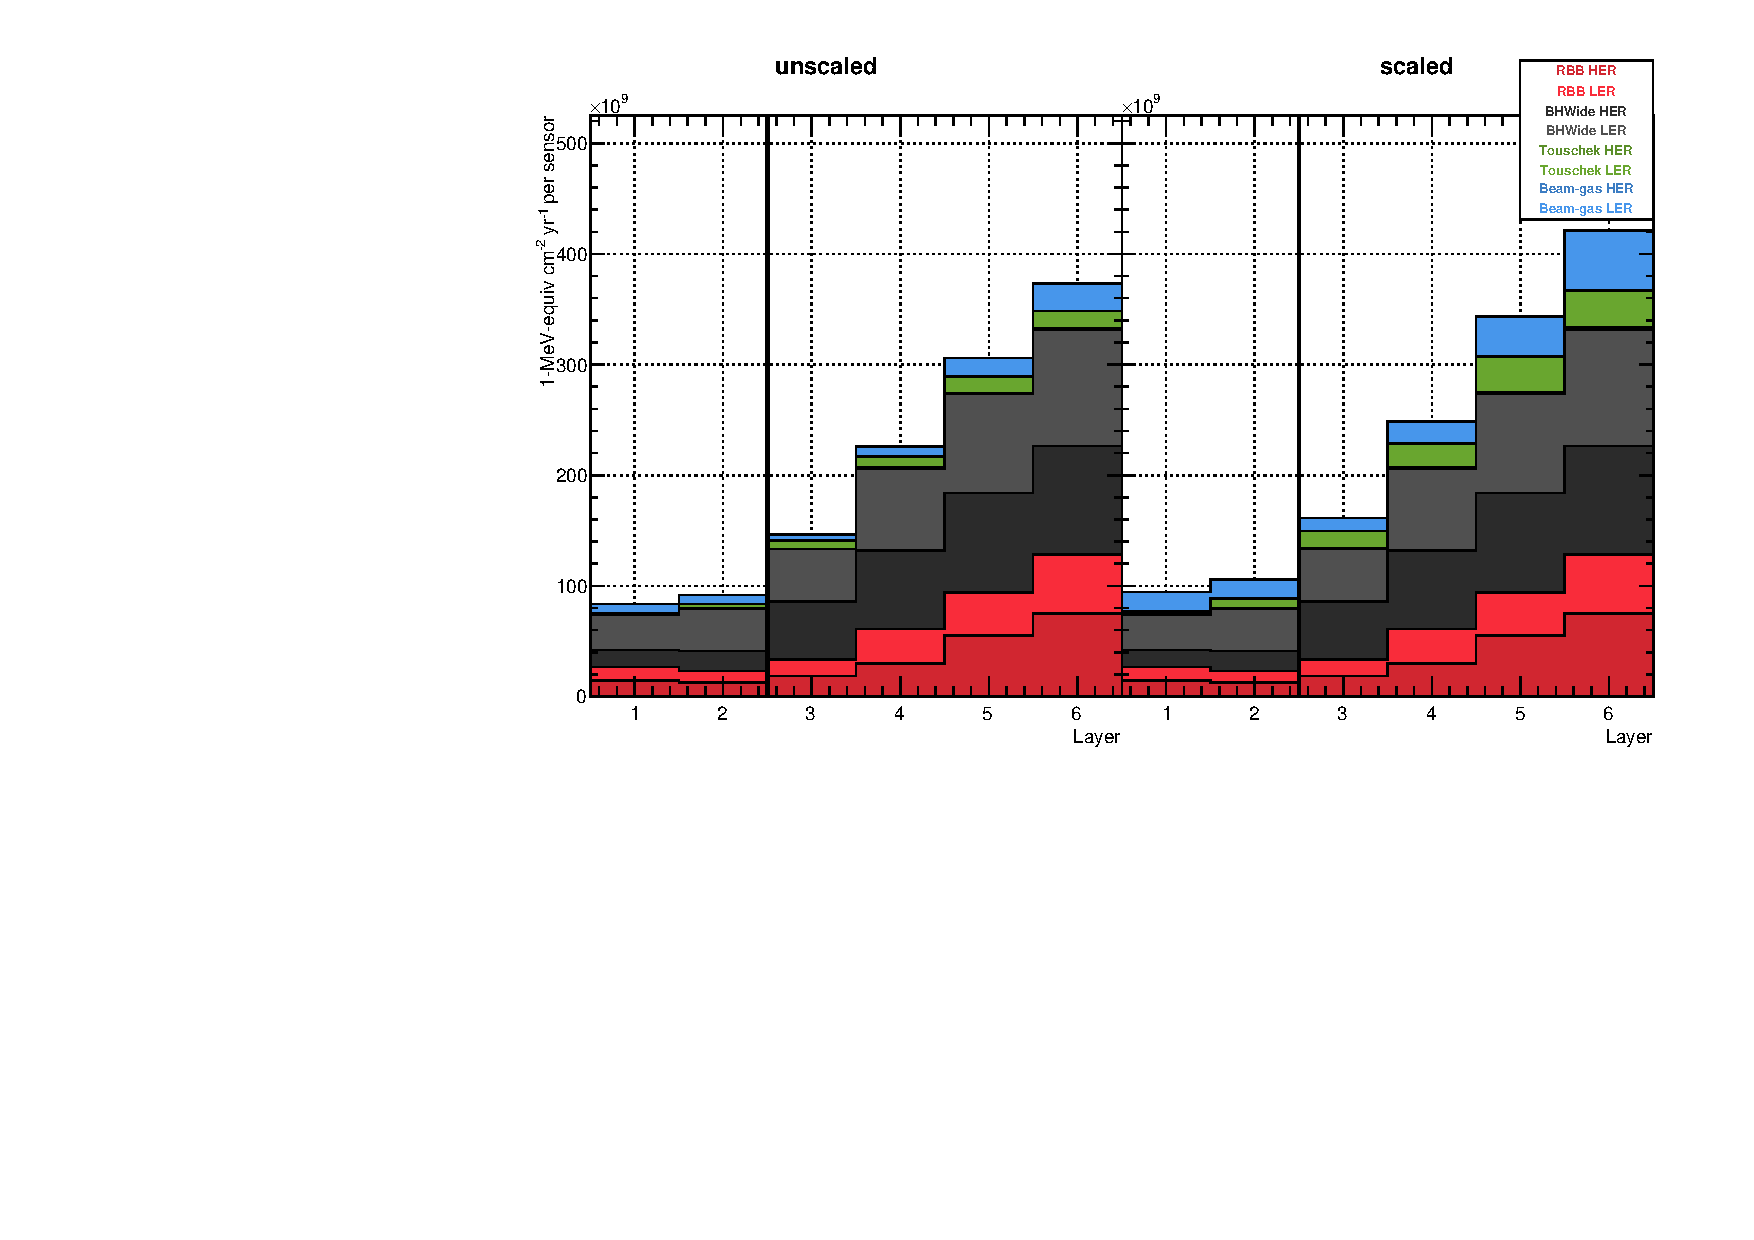
\includegraphics[width=\textwidth]{images/hVXDFlux}
	\caption[Neutron flux in VXD]{Neutron flux in VXD. Layers 1 \& 2 are the PXD and 3-6 are the SVD.}	
	\label{fig:VXDFlux}
\end{figure}

\begin{figure}[htb]
	\centerfloat
		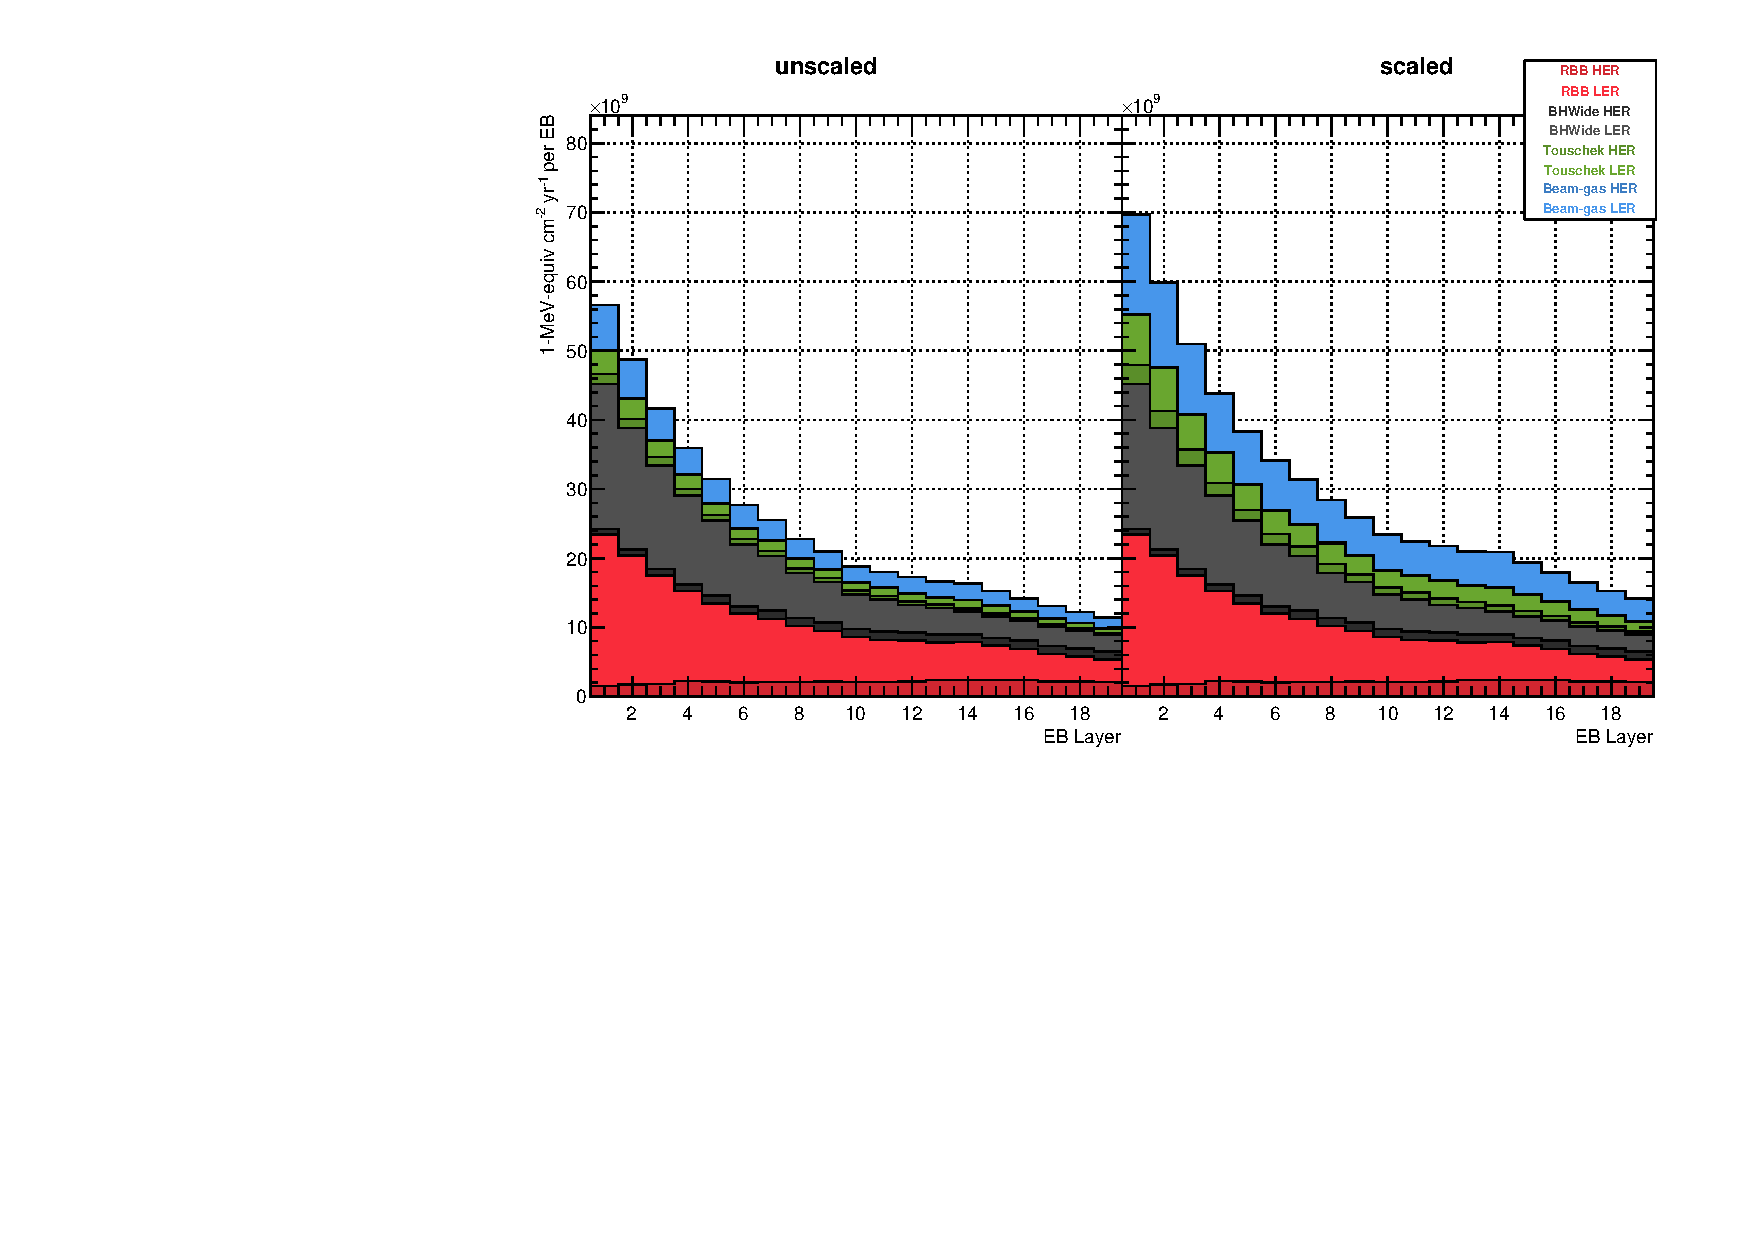
\includegraphics[width=\textwidth]{images/hCDCFlux}
	\caption[Neutron flux in CDC electronics]{Neutron flux in CDC electronics. Layer 1 is the innermost layer. Larger layer numbers correspond to higher radii.}	
	\label{fig:CDCFlux}
\end{figure}

\begin{figure}[htb]
	\centerfloat
		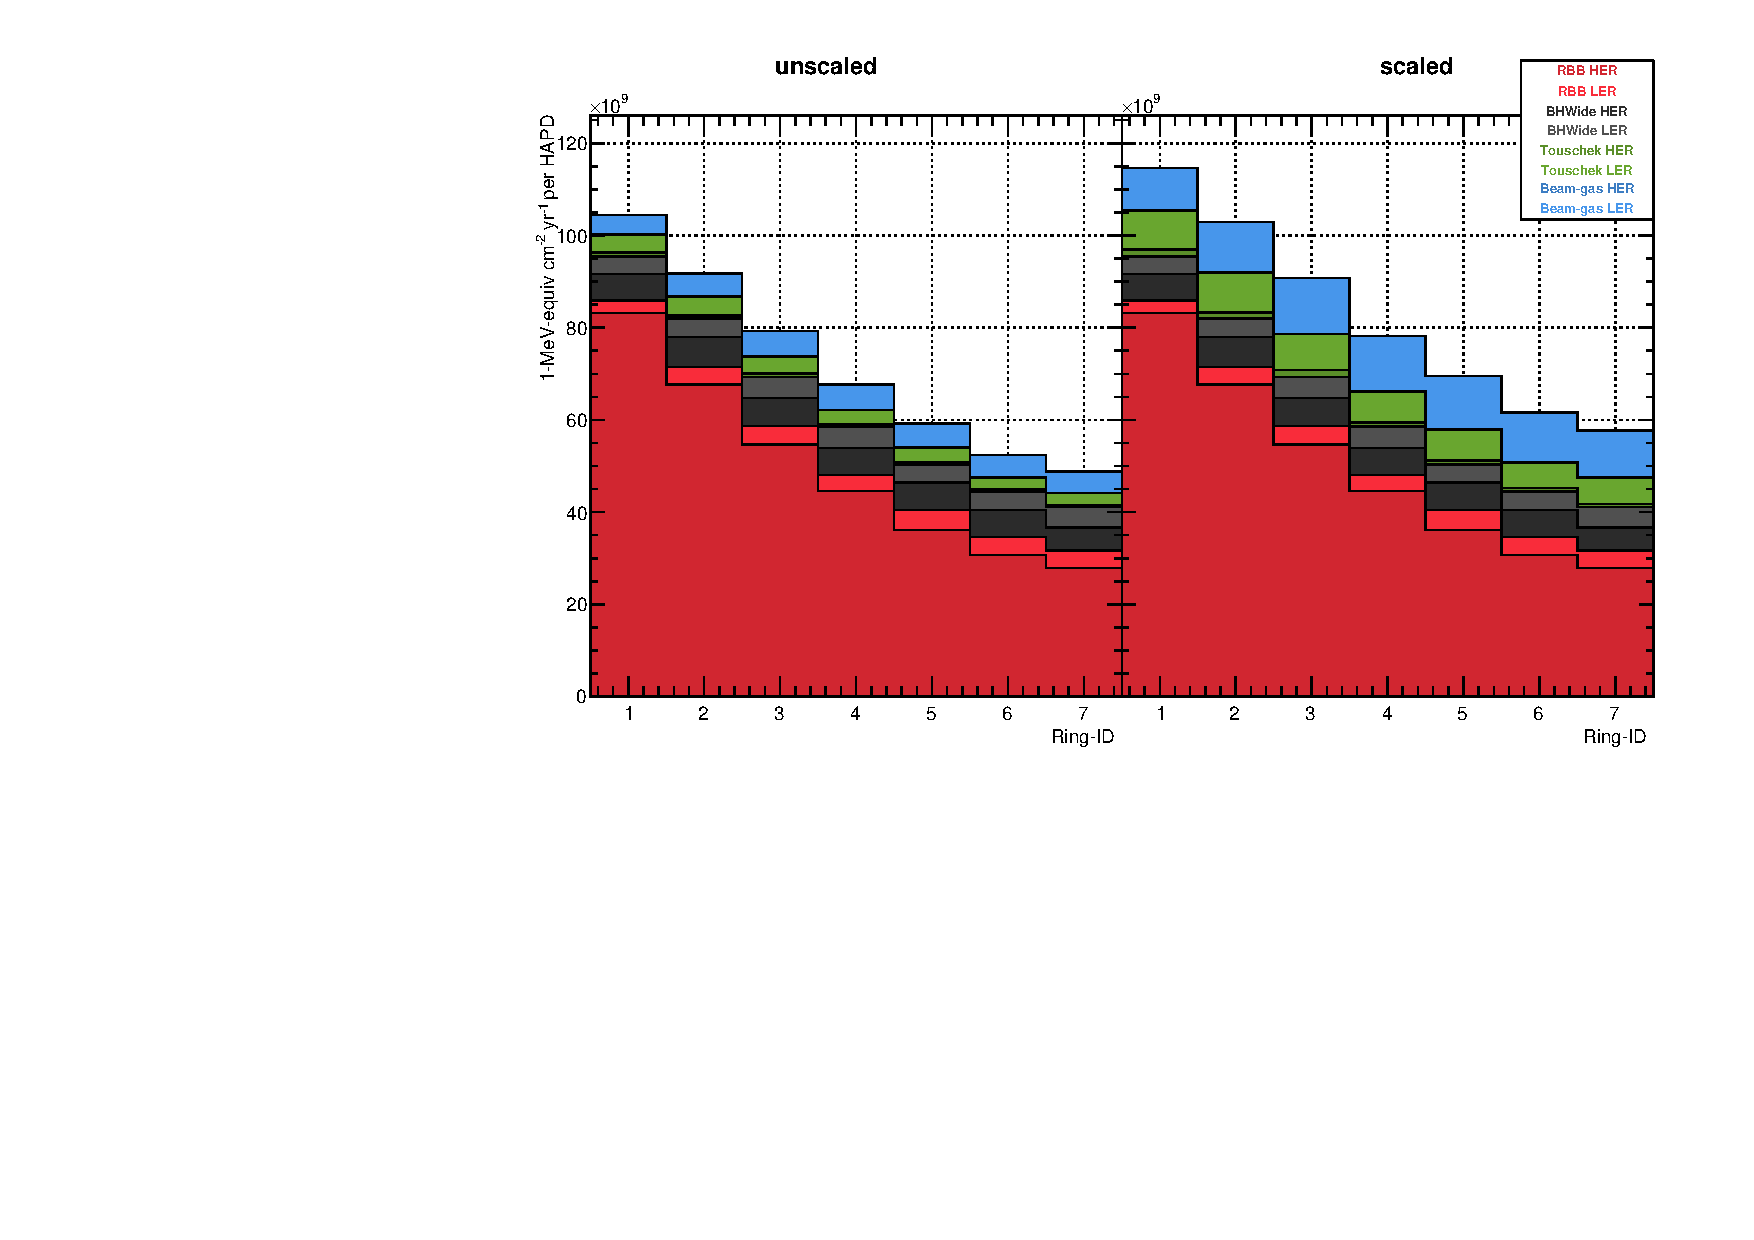
\includegraphics[width=\textwidth]{images/hARICHFlux}
	\caption[Neutron flux in ARICH rings]{Neutron flux in ARICH Rings. Ring-ID of 1 is the innermost ring. Ring-ID increases with radius.}	
	\label{fig:ARICHFlux}
\end{figure}

\begin{figure}[htb]
	\centerfloat
		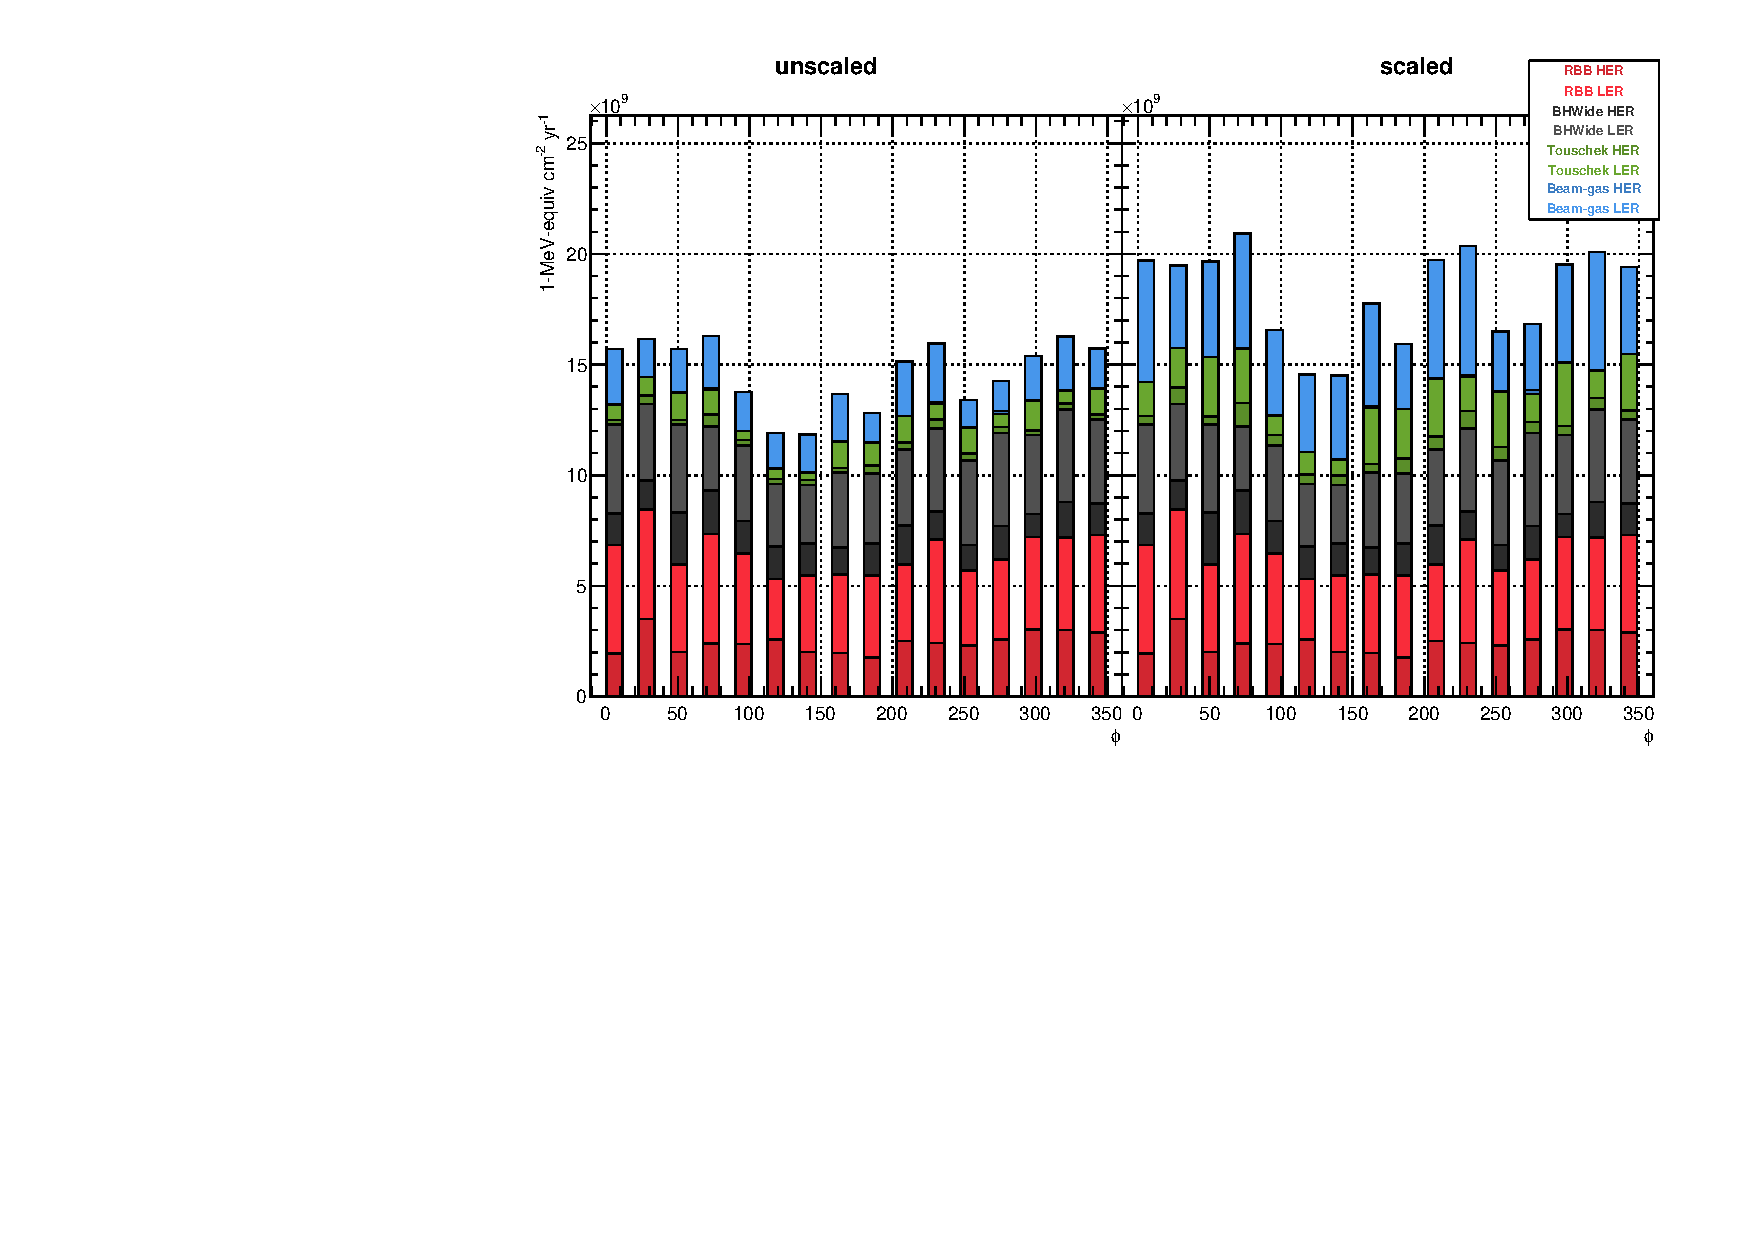
\includegraphics[width=\textwidth]{images/hTOPFlux}
	\caption{Neutron flux in TOP electronics.}	
	\label{fig:TOPFlux}
\end{figure}

\begin{figure}[htb]
	\centerfloat
		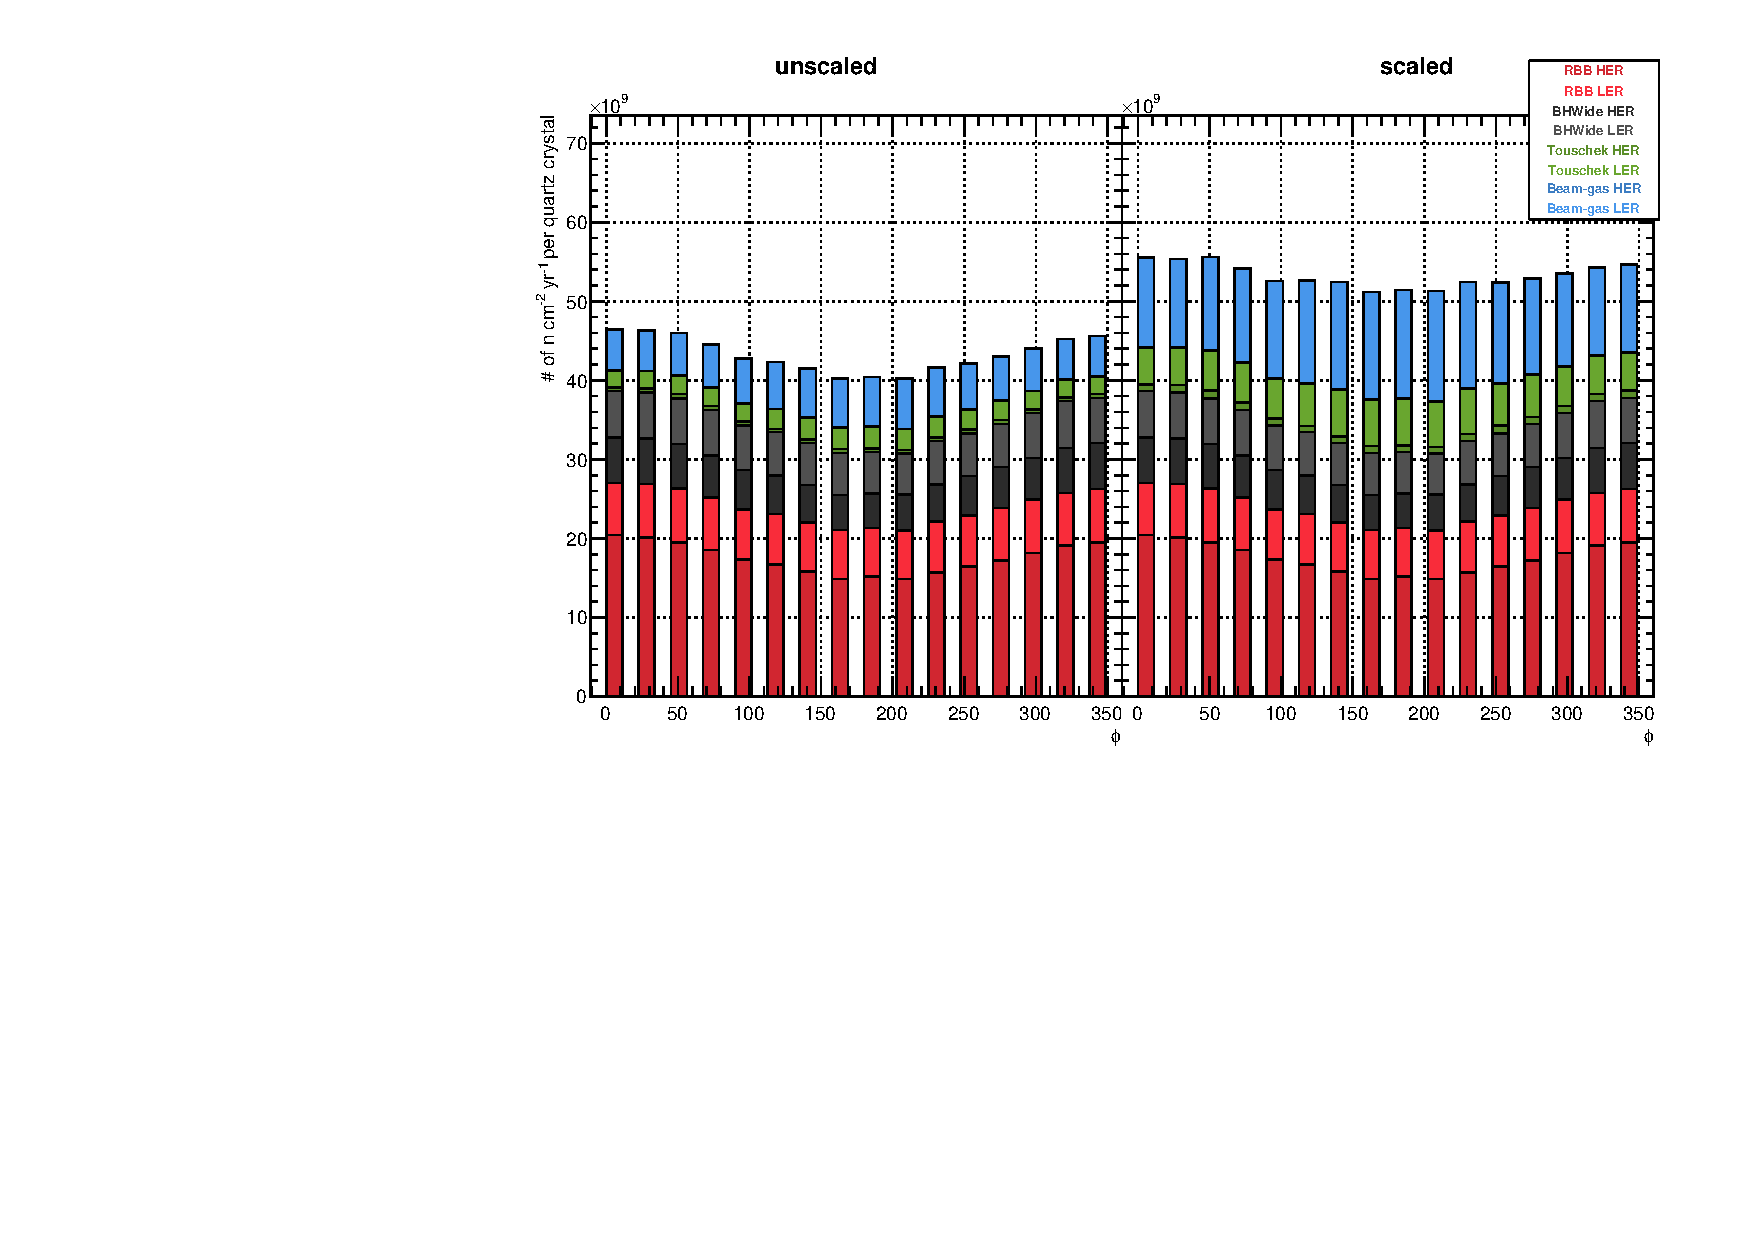
\includegraphics[width=\textwidth]{images/hTOPFluxBar}
	\caption{Neutron flux in TOP quartz bars.}	
	\label{fig:TOPBARFlux}
\end{figure}

\begin{figure}[htb]
	\centerfloat
		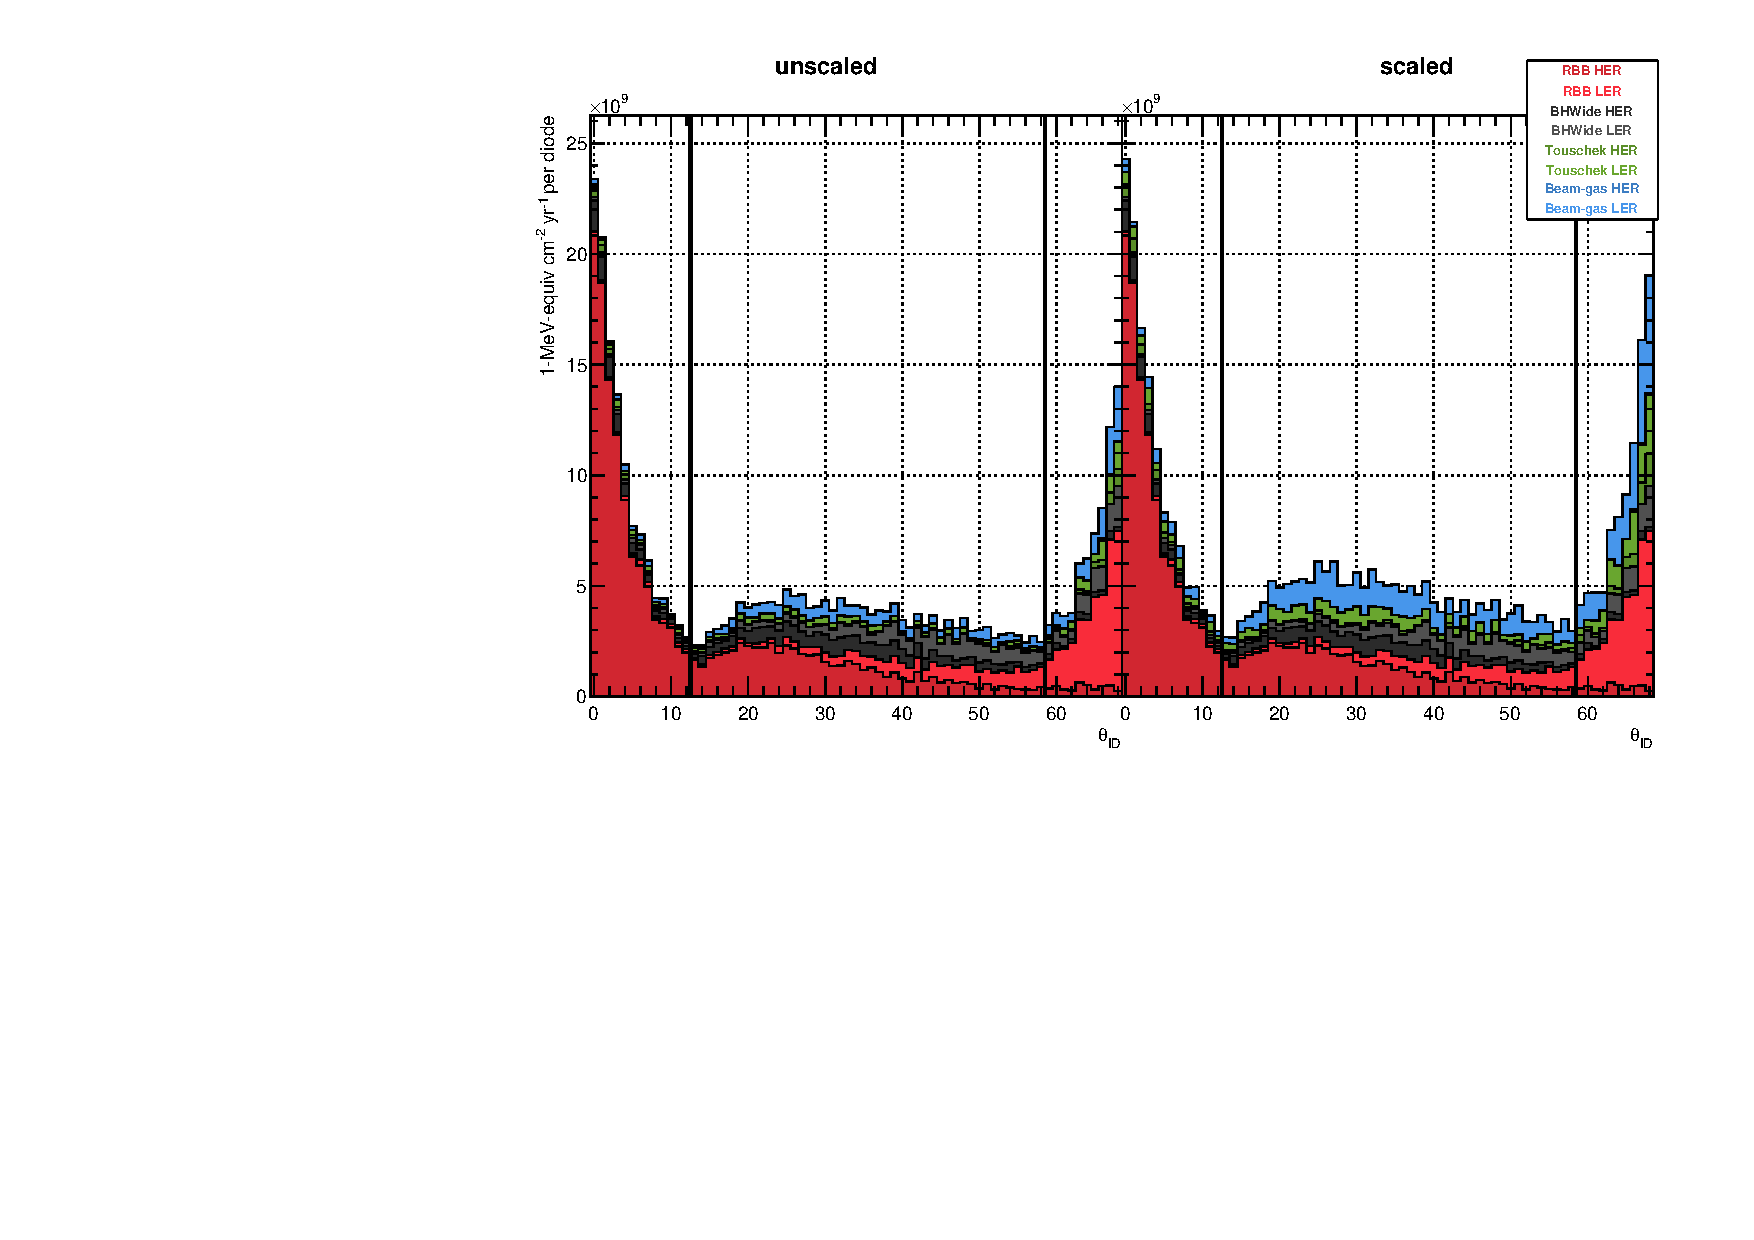
\includegraphics[width=\textwidth]{images/hECLFluxTID}
	\caption[Neutron flux in ECL diodes]{Neutron flux in ECL diodes. Explanation of $\theta_{ID}$ can be found in Appendix \ref{chap:THID}.}	
	\label{fig:ECLFlux}
\end{figure}

\begin{figure}[htb]
	\centerfloat
		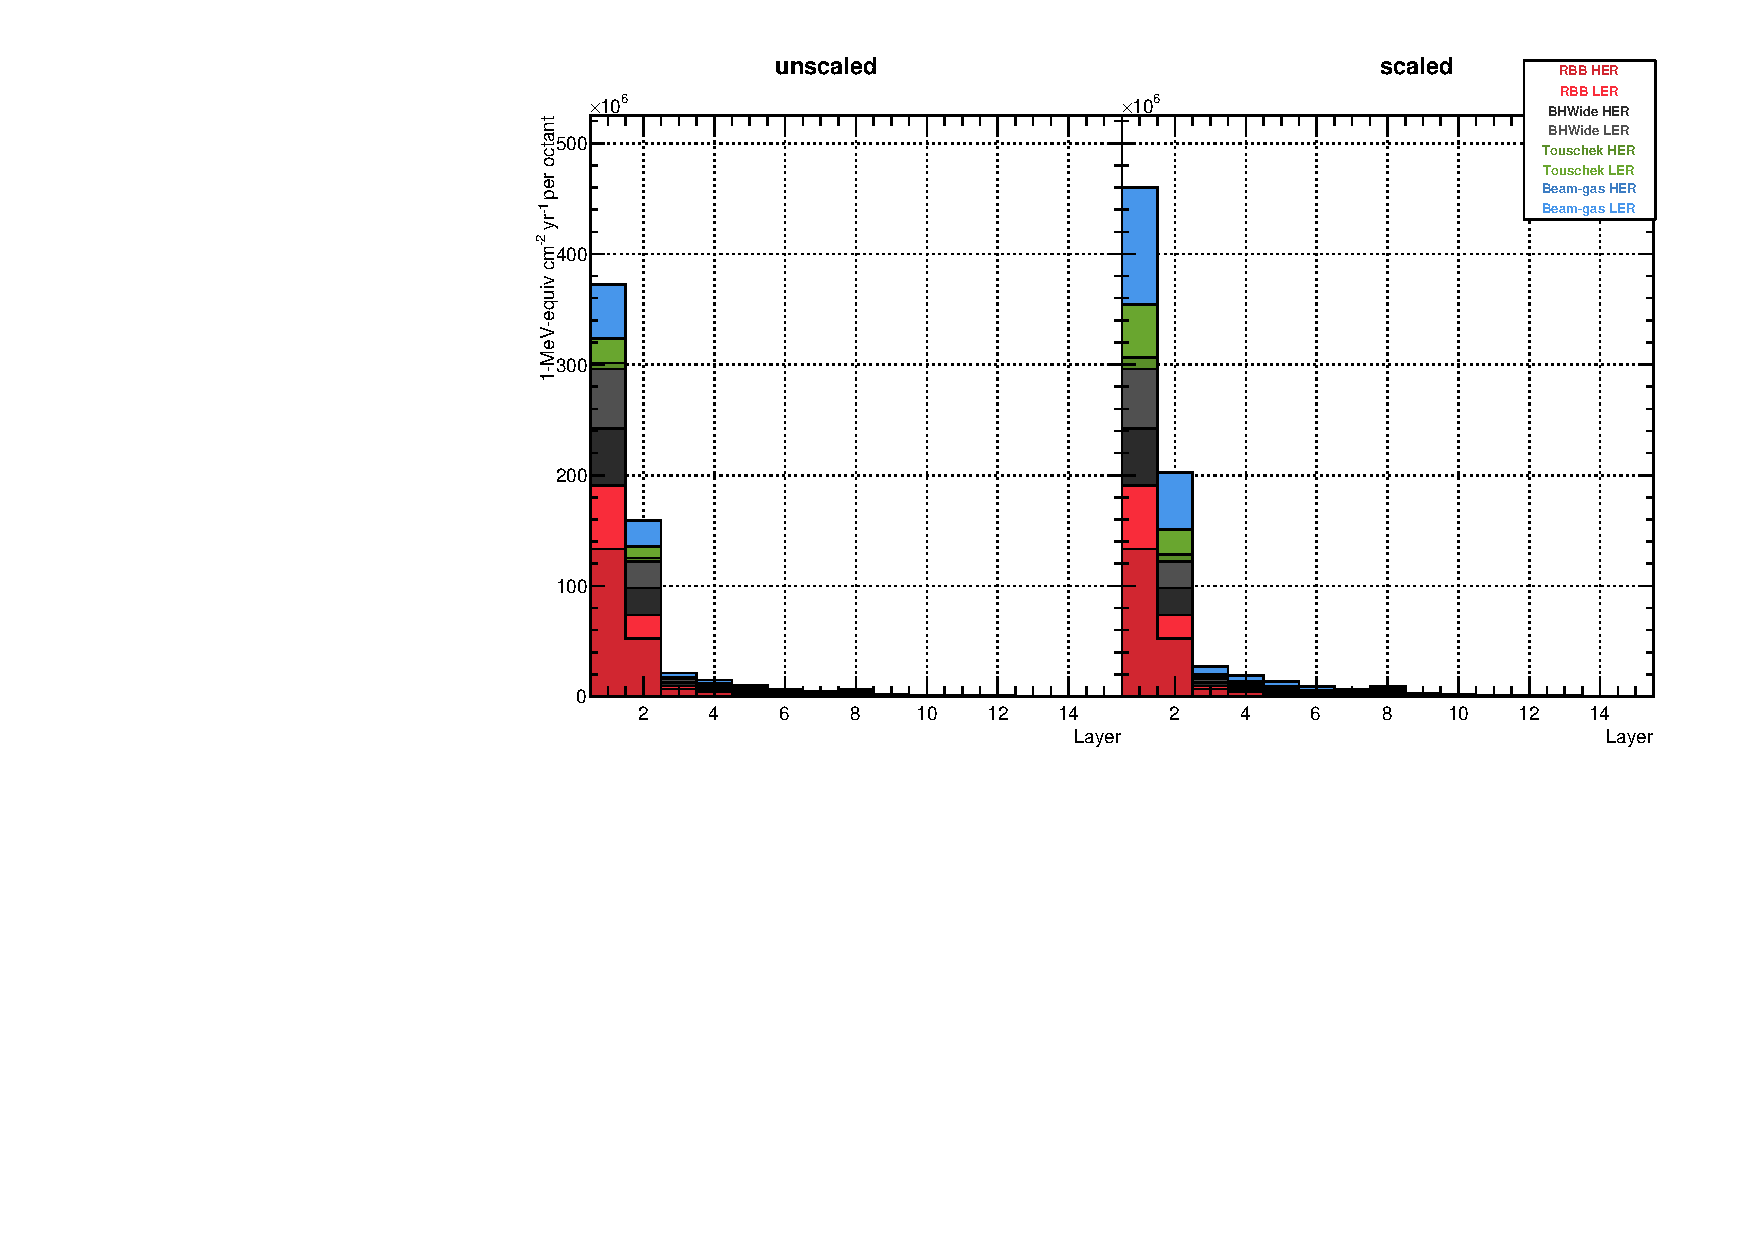
\includegraphics[width=\textwidth]{images/hBKLMFlux}
	\caption[Neutron flux in BKLM]{Neutron flux in BKLM. Layer 1 is the innermost layer. Layer increases with radius.}	
	\label{fig:BKLMFlux}
\end{figure}

\begin{figure}[htb]
	\centerfloat
		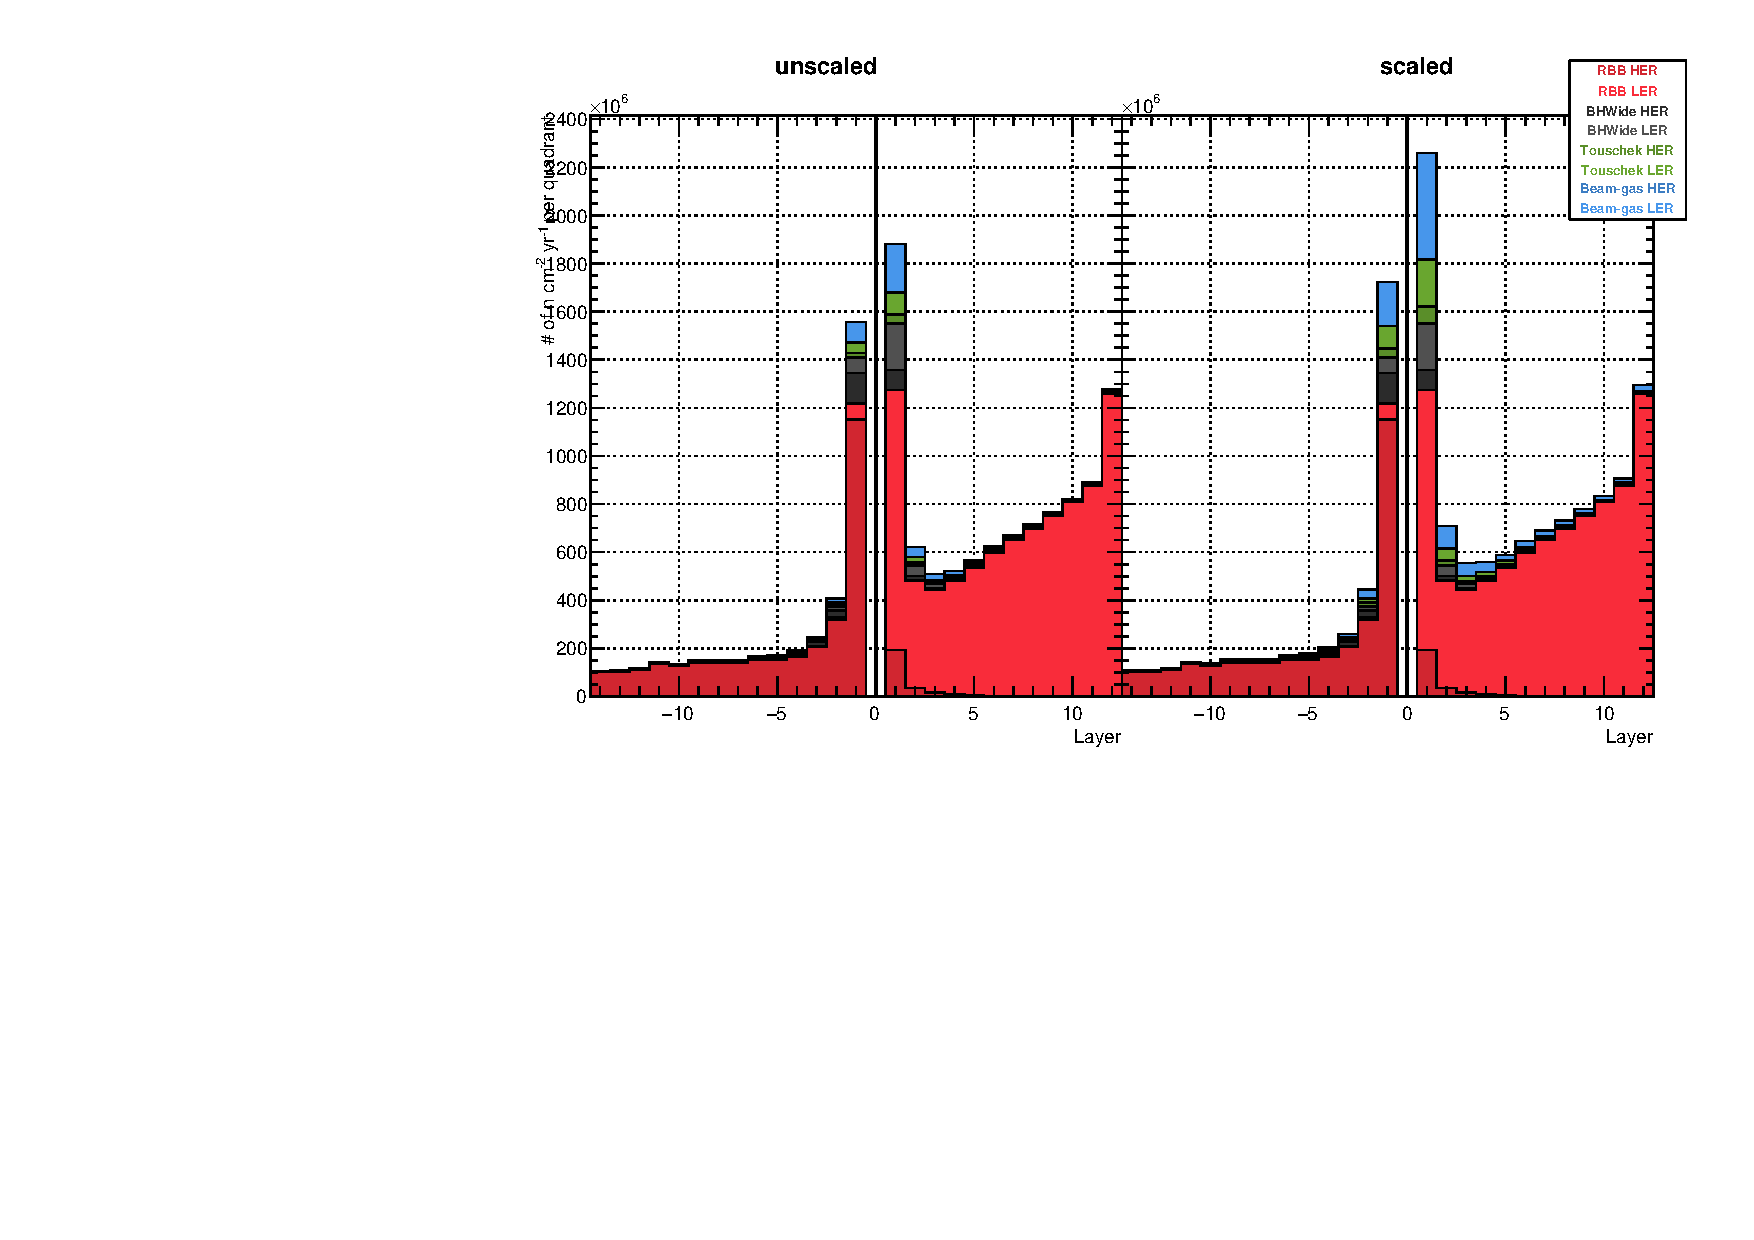
\includegraphics[width=\textwidth]{images/hEKLMFlux}
	\caption[Neutron flux in EKLM]{Neutron flux in EKLM. Negative layers are backward end-cap, positive layers are forward end-cap. Layers 1 and -1 are closest to IR.}	
	\label{fig:EKLMForFlux}
\end{figure}

%\begin{figure}[htb]
%	\centerfloat
%		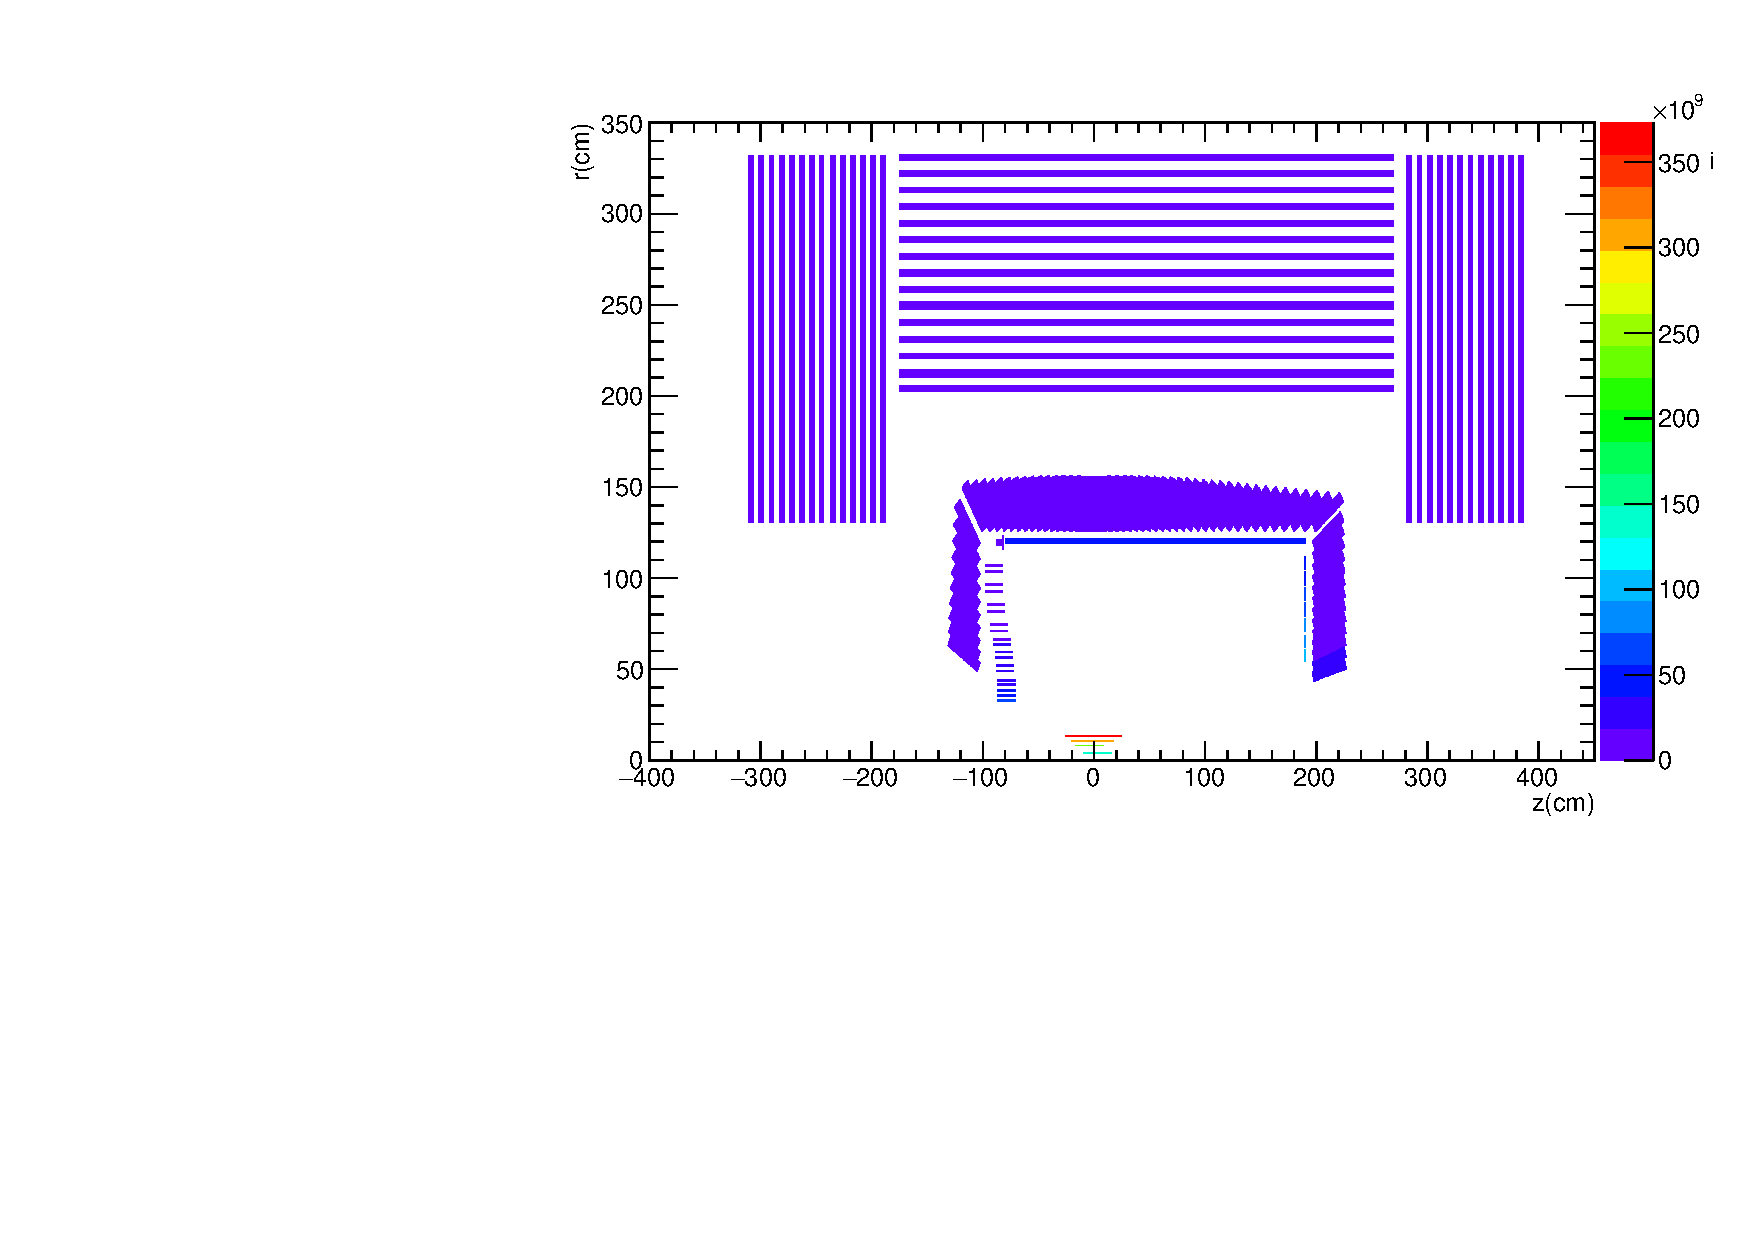
\includegraphics[scale=0.6]{images/BelleIIFlux}
%	\caption{Flux in the Belle~II detector}	
%	\label{fig:BelleIIFlux}
%\end{figure}


